%  !TeX  root  =  user_guide.tex

\chapter{功能速览}\label{feature_glance}

% when the revision of a section has been finalized,
% comment out the following line:
%\updatedisclaimer

章 \ref{label_getstarted}中对 \qg 功能进行了简单示范,下面将展开进行更加详尽的叙述。以下章节中提到的大部分功能将在文档各自相应的部分中得到解释和描述。

\section{启动和退出 \qg}\label{label_startinqgis}

在章 \ref{samplesession}中已经介绍了如何启动QGIS。这里我们将再重复一次,并且您将看到 \qg 还提供了更多的命令行选项。

\begin{itemize}
\item \nix{假设QGIS已经在PATH中安装,可通过以下方式启动QGIS:在命令提示符下键入 \usertext{qgis}或者在桌面或应用程序菜单中双击QGIS应用程序链接(或快捷方式)。}
\item \win{用开始菜单或桌面快捷方式打开QGIS或者双击QGIS工程文件。}
\item \osx{双击应用程序文件夹中的图标。 如果需要在Shell中启动QGIS,运行 /path-to-installation-executable/Contents/MacOS/Qgis。}
\end{itemize}

要停止 \qg,需要单击菜单项 \{\nix{}\win{File}\osx{QGIS}\} \arrow 退出,或者使用快捷键 \keystroke{Ctrl+Q}。

\subsection{命令行选项}\index{command line options}
\label{label_commandline}

\nix 从命令行启动时,QGIS支持很多命令选项。在命令行输入 \usertext{qgis ---help},就能看到一个选项列表。QGIS的用法说明是:

\small
\begin{verbatim}
qgis --help
Quantum GIS - 1.5.0-Tethys 'Tethys' (exported)
Quantum GIS (QGIS) is a viewer for spatial data sets, including
raster and vector data.
Usage: qgis [options] [FILES]
  options:
        [--snapshot filename]           emit snapshot of loaded datasets to given file
        [--width width]                 width of snapshot to emit
        [--height height]               height of snapshot to emit
        [--lang language]               use language for interface text
        [--project projectfile]         load the given QGIS project
        [--extent xmin,ymin,xmax,ymax]  set initial map extent
        [--nologo]                      hide splash screen
        [--noplugins]                   don't restore plugins on startup
        [--optionspath path]            use the given QSettings path
        [--configpath path]             use the given path for all user configuration
        [--help]                        this text

  FILES:
    Files specified on the command line can include rasters,
    vectors, and QGIS project files (.qgs):
     1. Rasters - Supported formats include GeoTiff, DEM
        and others supported by GDAL
     2. Vectors - Supported formats include ESRI Shapefiles
        and others supported by OGR and PostgreSQL layers using
        the PostGIS extension
\end{verbatim}
\normalsize

\begin{Tip} \caption{\textsc{使用命令行参数示例}}
您可以通过在命令行上指定一个或多个数据文件来启动QGIS。例如,假设您在qgis\_sample\_data目录中,就可以通过命令 \usertext{qgis ./raster/landcover.img ./gml/lakes.gml}在启动QGIS时加载一个矢量图层和一个栅格图层。
\end{Tip}

\minisec{命令行选项 \usertext{---snapshot}}
这个选项可以在当前窗口创建一个PNG格式的快照。当用户有很多项目并且想从数据中生成快照时,这就变得非常便利。

目前它能生成具有800×600像素的PNG文件。可用 \usertext{---width}和 \usertext{---height}命令行参数来完成。文件名可加在\usertext{---snapshot}之后。

\minisec{命令行选项 \usertext{---lang}}
根据情况QGIS选择需要的本地化语言。如果想改变语言可指定语言码。例如: \usertext{---lang=it}启动意大利版QGIS。\url{http://www.qgis.org/wiki/GUI_Translation_Progress}提供了目前所支持语言的代码和状态。

\minisec{命令行选项 \usertext{---project}}
也可以用QGIS启动一个现有的工程文件。只需要在工程名后添加 \usertext{--project},QGIS就可打开加载在给定文件中的所有图层。

\minisec{命令行选项 \usertext{---extent}}
打开一个特定的地图范围需要用到此选项。需要通过下面这个用逗号分开的命令来添加一个范围边界框:

\begin{verbatim}
--extent xmin,ymin,xmax,ymax
\end{verbatim}

\minisec{命令行选项 \usertext{---nologo}}
当启动QGIS时,此命令行参数隐藏启动画面。

\minisec{命令行选项 \usertext{---noplugins}}
如果QGIS带插件启动时出现问题,你可以在启动时取消加载插件。这些插件在之后从插件管理器中启用。

\minisec{命令行选项 \usertext{---optionspath}}
当你有不同的软件设置时,您可以使用本选项来决定使用哪一个配置文件启动QGIS。可以在章 \ref{subsec:gui_options}中查看操作系统保存设置文件的位置。到目前为止还不能设置配置文件的保存位置,所以您可以保存一份原始配置文件的副本并重命名。

\minisec{命令行选项 \usertext{---configpath}}
本选项和上一个选项类似,但是会修改默认的配置文件位置(~/.qgis)以进行用户自定义配置,并且还会强制Qt设置QSettings使用该配置目录。这就允许用户,比如,在闪存盘上安装QGIS及其插件和设置。

\section{QGIS GUI}\index{main window}
\label{label_qgismainwindow}

当启动QGIS时,可看到如下所示的GUI(黄色椭圆形中的数字1到6是指以下所讨论的六个主要界面区域):

\begin{figure}[ht]
   \centering
    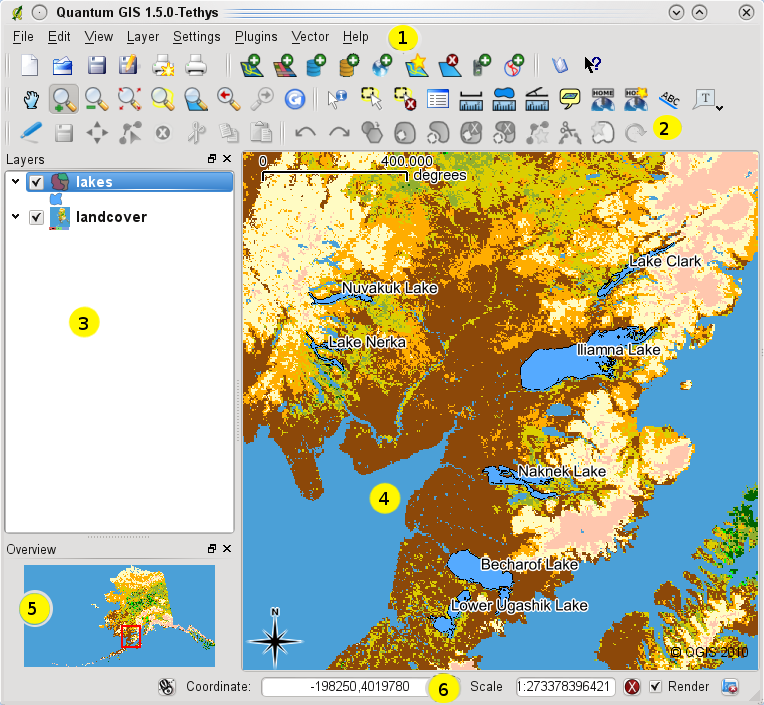
\includegraphics[clip=true, width=12cm]{startup}
    \caption{显示 Alaska 地区示例数据的 QGIS GUI \nixcaption (KDE)} \label{fig:startup}
\end{figure}

\textbf{注意:} 您的窗口装饰(标题栏等)可能因操作系统和窗口管理器的不同而不同。\\

QGIS GUI被划分为六个区域:

\begin{tabular}{p{5cm} p{5cm}}
%\centering
1. 菜单栏  & 4. 地图显示区 \\
2. 工具栏 & 5. 地图预览区 \\
3. 图例显示区 & 6. 状态栏 \\
\end{tabular}

下面各节对QGIS界面这六大部分进行了更加详尽的描述。还有两节介绍了键盘快捷键和上下文帮助。

% \newpage

\subsection{菜单栏}\label{label_menubar}
\index{menus}

菜单栏通过标准的分层菜单向用户提供了各种QGIS功能。下面列出了顶层菜单和一些菜单选项的汇总及其对应的工具栏上的图标和键盘快捷键。 \footnote{键盘快捷键现在可以手动配置(本节中给出快捷键是默认的版本),只需要点击设置菜单项下的自定义快捷键命令}虽然大部分菜单选项都有相应的工具,反之亦然,但是菜单并没有像工具栏一样安排有序。每次进入菜单选项选择复选框后工具栏中包含的所有工具都会被列出。更多关于工具和工具栏的信息详见章节 \ref{label_toolbars}。

\begin{tabbing}
\hspace{5.5cm}\=\hspace{3cm}\=\hspace{3.5cm}\= \kill
\hspace{1cm} 菜单选项 \> 快捷键 \> 参考章节 \> 工具栏\\
\end{tabbing}

\begin{itemize}
\item \mainmenuopt{文件}
\begin{tabbing}
\hspace{4.5cm}\=\hspace{3cm}\=\hspace{3.5cm}\= \kill
\dropmenuopttwo{mActionFileNew}{新建工程}
	\> \keystroke{Ctrl+N}
	\> 参见章 \ref{sec:projects}
	\> \dropmenucheck{文件} \\
\dropmenuopttwo{mActionFileOpen}{打开工程}
	\> \keystroke{Ctrl+O}
	\> 参见章 \ref{sec:projects}
	\> \dropmenucheck{文件} \\
\dropmenuopt{打开最近工程}
	\>
	\> 参见章 \ref{sec:projects} \\
\dropmenuopttwo{mActionFileSave}{保存工程}
	\> \keystroke{Ctrl+S}
	\> 参见章 \ref{sec:projects}
	\> \dropmenucheck{文件} \\
\dropmenuopttwo{mActionFileSaveAs}{工程另存为}
	\> \keystroke{Ctrl+Shift+S}
  \> 参见章 \ref{sec:projects}
	\> \dropmenucheck{文件} \\
\dropmenuopttwo{mActionSaveMapAsImage}{另存为图像}
	\>
	\> 参见章 \ref{sec:output} \\
\dropmenuopttwo{mActionNewComposer}{新建打印设置}
        \> \keystroke{Ctrl+P}
        \> 参见章 \ref{label_printcomposer}
        \> \dropmenucheck{文件} \\
\dropmenuopttwo{mActionComposerManager}{打印设置}
	\>
	\> 参见章 \ref{label_printcomposer}
	\> \dropmenucheck{文件} \\
\dropmenuopt{打印设置}
	\>
	\> 参见章 \ref{label_printcomposer} \\
\dropmenuopttwo{mActionFileExit}{退出}
	\> \keystroke{Ctrl+Q} \\
\end{tabbing}

\item \mainmenuopt{编辑}
\begin{tabbing}
\hspace{4.5cm}\=\hspace{3cm}\=\hspace{3.5cm}\= \kill
\dropmenuopttwo{mActionUndo}{撤销}
        \> \keystroke{Ctrl+Z}
        \> 参见章 \ref{sec:advanced_edit}
        \> \dropmenucheck{高级数字化} \\
\dropmenuopttwo{mActionRedo}{重做}
        \> \keystroke{Ctrl+Shift+Z}
        \> 参见章 \ref{sec:advanced_edit}
        \> \dropmenucheck{高级数字化} \\
\dropmenuopttwo{mActionEditCut}{图元剪切}
	\> \keystroke{Ctrl+X}
	\> 参见章 \ref{sec:edit_existing_layer}
	\> \dropmenucheck{数字化} \\
\dropmenuopttwo{mActionEditCopy}{图元复制}
	\> \keystroke{Ctrl+C}
	\> 参见章 \ref{sec:edit_existing_layer}
	\> \dropmenucheck{数字化} \\
\dropmenuopttwo{mActionEditPaste}{图元粘贴}
	\> \keystroke{Ctrl+V}
	\> 参见章 \ref{sec:edit_existing_layer}
	\> \dropmenucheck{数字化} \\
\dropmenuopttwo{mActionEditPaste}{图元移动}
        \>
        \> 参见章 \ref{sec:edit_existing_layer}
        \> \dropmenucheck{数字化} \\
\dropmenuopttwo{mActionDeleteSelected}{删除选中图元}
        \>
        \> 参见章 \ref{sec:edit_existing_layer}
        \> \dropmenucheck{数字化} \\
\dropmenuopttwo{mActionSimplify}{图元简化}
        \>
        \> 参见章 \ref{sec:advanced_edit}
        \> \dropmenucheck{高级数字化} \\
\dropmenuopttwo{mActionAddRing}{添加环}
        \>
        \> 参见章 \ref{sec:advanced_edit}
        \> \dropmenucheck{高级数字化} \\
\dropmenuopttwo{mActionAddIsland}{添加部分}
        \>
        \> 参见章 \ref{sec:advanced_edit}
        \> \dropmenucheck{高级数字化} \\
\dropmenuopttwo{mActionDeleteRing}{删除环}
        \>
        \> 参见章 \ref{sec:advanced_edit}
        \> \dropmenucheck{高级数字化} \\
\dropmenuopttwo{mActionDeletePart}{删除部分}
        \>
        \> 参见章 \ref{sec:advanced_edit}
        \> \dropmenucheck{高级数字化} \\
\dropmenuopttwo{mActionReshape}{图元调整}
        \>
        \> 参见章 \ref{sec:advanced_edit}
        \> \dropmenucheck{高级数字化} \\
\dropmenuopttwo{mActionSplitFeatures}{图元分割}
        \>
        \> 参见章 \ref{sec:advanced_edit}
        \> \dropmenucheck{高级数字化} \\
\dropmenuopttwo{mActionMergeFeatures}{合并选中图元}
        \>
        \> 参见章 \ref{sec:advanced_edit}
        \> \dropmenucheck{高级数字化} \\
\dropmenuopttwo{mActionNodeTool}{结点工具}
        \>
        \> 参见章 \ref{sec:edit_existing_layer}
        \> \dropmenucheck{数字化} \\
\dropmenuopttwo{mActionRotatePointSymbols}{旋转点状符号}
        \>
        \> 参见章 \ref{sec:advanced_edit}
        \> \dropmenucheck{高级数字化} \\
\end{tabbing}

在对图层激活 \toolbtntwo{mActionToggleEditing}{启动编辑} 工具后,您会在菜单 \mainmenuopt{编辑} 下发现一个捕捉图元的图标,具体取决于图层类型(点,线或面)。\\

\begin{tabbing}
\hspace{4.5cm}\=\hspace{3cm}\=\hspace{3.5cm}\= \kill
\dropmenuopttwo{mActionCapturePoint}{点捕捉}
        \>
        \> 参见章 \ref{sec:edit_existing_layer}
        \> \dropmenucheck{数字化} \\
\dropmenuopttwo{mActionCaptureLine}{线捕捉}
        \>
        \> 参见章 \ref{sec:edit_existing_layer}
        \> \dropmenucheck{数字化} \\
\dropmenuopttwo{mActionCapturePolygon}{多边形捕捉}
        \>
        \> 参见章 \ref{sec:edit_existing_layer}
        \> \dropmenucheck{数字化} \\
\end{tabbing}


\item \mainmenuopt{视图}
\begin{tabbing}
\hspace{4.5cm}\=\hspace{3cm}\=\hspace{3.5cm}\= \kill
\dropmenuopttwo{mActionPan}{地图漫游}
	\>
	\> \> \dropmenucheck{地图导航} \\
\dropmenuopttwo{mActionZoomIn}{地图放大}
	\> \keystroke{Ctrl++}
	\> \> \dropmenucheck{地图导航} \\
\dropmenuopttwo{mActionZoomOut}{地图缩小}
	\> \keystroke{Ctrl+-}
	\> \> \dropmenucheck{地图导航} \\
\dropmenuopttwo{mActionSelect}{图元选择}
	\> 
	\> 参见章 \ref{sec:selection} 
	\> \dropmenucheck{属性} \\
\dropmenuopttwo{mActionDeselectAll}{取消所有选中图元}
        \>
        \> \> \dropmenucheck{属性} \\
\dropmenuopttwo{mActionIdentify}{图元标记}
	\> \keystroke{Ctrl-Alt-I}
	\> \> \dropmenucheck{属性} \\
\dropmenuopttwo{mActionMeasure}{直线量测}
	\> \keystroke{Ctrl-Alt-M}
	\> \> \dropmenucheck{属性} \\
\dropmenuopttwo{mActionMeasureArea}{面积量测}
	\> \keystroke{Ctrl-Alt-J}
	\> \> \dropmenucheck{属性} \\
\dropmenuopttwo{mActionMeasureAngle}{角度量测}
	\>
	\> \> \dropmenucheck{属性} \\
\dropmenuopttwo{mActionOpenTable}{按屏幕缩放}
	\> \keystroke{Ctrl-Alt-F}
	\> \> \dropmenucheck{地图导航} \\
\dropmenuopttwo{mActionZoomToLayer}{按图层缩放}
	\>
	\> \> \dropmenucheck{地图导航} \\
\dropmenuopttwo{mActionZoomToSelected}{按选择区缩放}
	\> \keystroke{Ctrl+J}
	\> \> \dropmenucheck{地图导航} \\
\dropmenuopttwo{mActionZoomLast}{返回最后一次缩放}
	\>
	\> \> \dropmenucheck{地图导航} \\
\dropmenuopttwo{mActionZoomNext}{重做下一次缩放}
	\>
	\> \> \dropmenucheck{地图导航} \\
\mainmenuopt{按实际大小缩放}
	\>
	\> \>  \\
\dropmenuopttwo{mActionMapTips}{地图小技巧}
	\>
	\> \> \dropmenucheck{属性} \\
\dropmenuopttwo{mActionNewBookmark}{新建书签}
	\> \keystroke{Ctrl+B}
	\> 参见章 \ref{sec:bookmarks}
\> \dropmenucheck{属性} \\
\dropmenuopttwo{mActionShowBookmarks}{显示书签}
	\> \keystroke{Ctrl-Alt-B}
	\> 参见章 \ref{sec:bookmarks}
	\> \dropmenucheck{属性} \\
\dropmenuopttwo{mActionDraw}{刷新}
	\> \keystroke{Ctrl+R}
	\> \> \dropmenucheck{地图导航} \\
\mainmenuopt{平铺缩放条}
	\>
	\> 参见章 \ref{sec:tilesets}
	\> \dropmenucheck{平铺缩放条} \\
\mainmenuopt{Live GPS tracking}
	\>
	\> 参见章 \ref{sec:gpstracking}
	\> \dropmenucheck{GPS 信息} \\
\end{tabbing}

\item \mainmenuopt{图层}
\begin{tabbing}
\hspace{5cm}\=\hspace{3cm}\=\hspace{3.5cm}\= \kill
\dropmenuopt{新建}
	\>
	\> 参见章 \ref{sec:create shape}
	\> \dropmenucheck{图层管理} \\
\mainmenuopt{栅格图层计算}
        \>
        \> 参见章 \ref{sec:raster_calc}
        \>  \\
\dropmenuopttwo{mActionAddNonDbLayer}{添加矢量图层}
	\> \keystroke{Ctrl+Shift+V}
	\>
	参见章 \ref{label_workingvector}
	\> \dropmenucheck{图层管理} \\
\dropmenuopttwo{mActionAddRasterLayer}{添加栅格图层}
	\> \keystroke{Ctrl+Shift+R}
	\>
	参见章 \ref{label_raster}
	\> \dropmenucheck{图层管理} \\
\dropmenuopttwo{mActionAddLayer}{添加PostGIS图层}
	\> \keystroke{Ctrl+Shift+D}
	\>
	参见章 \ref{label_postgis}
        \> \dropmenucheck{图层管理} \\
\dropmenuopttwo{mActionAddSpatiaLiteLayer}{添加SpatiaLite图层}
        \> \keystroke{Ctrl+Shift+L}
        \>
        参见章 \ref{label_spatialite}
	\> \dropmenucheck{图层管理} \\
\dropmenuopttwo{mActionAddWmsLayer}{添加WMS图层}
	\> \keystroke{Ctrl+Shift+W}
	\>
	参见章 \ref{sec:ogc-wms}
	\> \dropmenucheck{图层管理} \\
\dropmenuopttwo{mActionOpenTable}{打开属性表}
	\> \>
	\> \dropmenucheck{属性} \\
\dropmenuopttwo{mActionFileSave}{保存修改}
        \> \>
        \> \dropmenucheck{数字化} \\
\dropmenuopttwo{mActionToggleEditing}{启动编辑状态}
	\> \>
	\> \dropmenucheck{数字化} \\
\mainmenuopt{另存为。。。}
	\\
\mainmenuopt{选区另存为矢量图层。。。}
	\> 
	\> See \ref{sec:attribute table}
	\> \\
\dropmenuopttwo{mActionRemoveLayer}{移除图层}
	\> \keystroke{Ctrl+D}
	\>
	\> \dropmenucheck{特性} \\
\mainmenuopt{特性}
	\\
\mainmenuopt{查询。。。}
	\\
\dropmenuopttwo{mActionInOverview}{添加到预览}
	\> \keystroke{Ctrl+Shift+O}
	\>
	\> \dropmenucheck{图层管理} \\
\dropmenuopttwo{mActionAddAllToOverview}{全部添加到预览}
	\>
	\>
	\\
\dropmenuopttwo{mActionRemoveAllFromOverview}{从预览移除全部}
	\>
	\>
	\\
\dropmenuopttwo{mActionHideAllLayers}{隐藏所有图层}
	\> \keystroke{Ctrl+Shift+H}
	\>
	\> \dropmenucheck{图层管理} \\
\dropmenuopttwo{mActionShowAllLayers}{显示所有图层}
	\> \keystroke{Ctrl+Shift+U}
	\>
	\> \dropmenucheck{图层管理} \\
\dropmenuopttwo{labeling}{标注}
	\>
	\>
	\\
\end{tabbing}

\item \mainmenuopt{设置}
\begin{tabbing}
\hspace{5cm}\=\hspace{3cm}\=\hspace{3.5cm}\= \kill
\dropmenuopt{面板}
	\>
	\>
	\\
\dropmenuopt{工具栏}
	\>
	\>
	\\
\mainmenuopt{启动全屏模式}
	\>\keystroke{Ctrl-F}
	\>
	\\
\dropmenuopttwo{mActionProjectProperties}{工程设置}
	\> \keystroke{Ctrl-Alt-P}
	\> 参见章 \ref{sec:projects} \\
\dropmenuopttwo{mActionCustomProjection}{自定义CRS}
        \> \> 参见章 \ref{sec:customprojections} \\
\mainmenuopt{样式管理}
        \> \> \\
\dropmenuopttwo{mActionOptions}{自定义快捷键}
        \> \> \\
\dropmenuopttwo{mActionOptions}{选项}
        \> \> 参见章 \ref{subsec:gui_options} \\
\end{tabbing}

\item \mainmenuopt{插件} - (添加由插件扩展的菜单项。)
\begin{tabbing}
\hspace{5cm}\=\hspace{3cm}\=\hspace{3.5cm}\= \kill
\dropmenuopttwo{mActionShowPluginManager}{插件管理}
	\> \> 参见章 \ref{sec:managing_plugins} \dropmenucheck{插件}
	\\
	\mainmenuopt{Python终端}
        \> \>
        \\
\end{tabbing}

\item \mainmenuopt{帮助}
\begin{tabbing}
\hspace{5cm}\=\hspace{3cm}\=\hspace{3.5cm}\= \kill
\dropmenuopttwo{mActionHelpContents}{帮助上下文}
	\> \keystroke{F1}
	\>
	\> \dropmenucheck{帮助}\\
\dropmenuopttwo{mActionQgisHomePage}{QGIS主页}
	\> \keystroke{Ctrl+H}
	\>
	\\
\dropmenuopttwo{mActionCheckQgisVersion}{查看QGIS版本}
	\\
\dropmenuopttwo{mActionHelpAbout}{关于}
	\\
\end{tabbing}

\end{itemize}

\textbf{注意:} \nix 上面列出的菜单栏项在KDE窗口管理器中都是默认的。在GNOME中没在“设置”菜单项,但在以下这些地方可以找到:

\begin{tabbing}
\dropmenuopttwo{mActionProjectProperties}{工程设置} \hspace{3cm}\=
\dropmenucheck{文件菜单} \\
\dropmenuopttwo{mActionOptions}{选项} \hspace{3cm}\>
\dropmenucheck{编辑}\\
\dropmenuopttwo{mActionOptions}{自定义快捷键} \hspace{3cm}\>
\dropmenucheck{编辑}\\
\mainmenuopt{样式管理} \hspace{3cm}\>
\dropmenucheck{编辑}\\
\dropmenuopttwo{mActionCustomProjection}{自定义CRS}\hspace{3cm}\>
\dropmenucheck{编辑} \\
\dropmenuopt{面板} \hspace{3cm}\>
\dropmenucheck{视图} \\
\dropmenuopt{工具栏}   \hspace{3cm}\>
\dropmenucheck{视图} \\
\mainmenuopt{启动全屏模式} \hspace{3cm}\>
\dropmenucheck{视图} \\
\mainmenuopt{平铺缩放条} \hspace{3cm}\>
\dropmenucheck{视图} \\
\mainmenuopt{GPS实时跟踪} \hspace{3cm}\>
\dropmenucheck{视图} \\
\end{tabbing}

%See Appendix \ref{app_menu} for complete descriptions of the menu items.

\subsection{工具栏}\label{label_toolbars}
\index{toolbars}

工具栏提供了大部分与菜单相同的功能,另外还提供了与地图进行交互访问的工具。每个工具栏项都可弹出帮助,将鼠标停留在工具项上就会显示该工具的简单描述。
每个菜单条都可以据需要而移动。另外,在工具栏点击鼠标右键显示快捷菜单可选择关闭菜单条。

\begin{Tip}
\caption{\textsc{重置工具栏}} \index{layout!toolbars}
如果不小心隐藏所有工具栏,可以选择 \mainmenuopt{设置} \arrow \dropmenuopt{工具栏} 使之再度出现。
\end{Tip}

\subsection{图例显示区}\label{label_legend}
\index{legend}

地图图例区用于设置图层可见性和叠置次序。叠置顺序是指接近说明顶层的图层在较低层的图层之上。每个说明条目的复选框都可用于显示或者隐藏图层。\index{layer!visibility}
在地图图例窗口的图层可以通过增加一个图层组或者接拖拽图层到一个组而对图层进行分组。操作如下,移动鼠标指针到图例窗口,点击右键,选择 \dropmenuopt{添加图层组} ,一个新的文件夹就出现。然后将图层拖到文件夹标志处。那么只需点击一次就可看到该组所有图层。鼠标右键点击图层标志选择 \dropmenuopt{移至最顶级} ,就将图层移出该组。在组右键菜单选择 \dropmenuopt{重命名} 对文件夹重新命名。
鼠标右键菜单目录取决于鼠标停在所加载的图例是栅格还是矢量图层。对于GRASS矢量图层,是不可用的。关于GRASS矢量图层的信息详见章节 \ref{grass_digitising} 。

\begin{itemize}

\item \textbf{栅格图层的右键菜单}
\begin{itemize}
\item \dropmenuopt{按图层边界缩放}
\item \dropmenuopt{按最佳比例缩放(100\%)}
\item \dropmenuopt{显示预览}
\item \dropmenuopt{移除}
\item \dropmenuopt{图层属性}
\item \dropmenuopt{重命名}
\item \dropmenuopt{添加图层组}
\item \dropmenuopt{展开全部}
\item \dropmenuopt{收起全部}
%%\item \dropmenuopt{Show file groups}
\end{itemize}

\item \textbf{矢量图层的右键菜单}
\begin{itemize}
\item \dropmenuopt{按图层边界缩放}
\item \dropmenuopt{显示预览}
\item \dropmenuopt{移除}
\item \dropmenuopt{打开属性表}
\item \dropmenuopt{开始编辑(对 GRASS 图层不可用)}
\item \dropmenuopt{另存为}
\item \dropmenuopt{选区另存为}
\item \dropmenuopt{查询}
\item \dropmenuopt{图层特性}
%% \item \dropmenuopt{Make to toplevel item}
\item \dropmenuopt{重命名}
\item \dropmenuopt{添加图层组}
\item \dropmenuopt{展开全部}
\item \dropmenuopt{收起全部}
%%\item \dropmenuopt{Show file groups}
\end{itemize}

\item \textbf{矢量图层的右键菜单}
\begin{itemize}
\item \dropmenuopt{移除}
\item \dropmenuopt{重命名}
\item \dropmenuopt{添加图层组}
\item \dropmenuopt{展开全部}
\item \dropmenuopt{收起全部}
%%\item \dropmenuopt{Show file groups}
\end{itemize}

\end{itemize}

如果几个矢量数据源有相同的矢量类型和属性,那么它们的符号可被分组。也就是说如果一个数据源的符号改变,则其他几个也作出改变。在图例窗口中打开右键菜单选择 \dropmenuopt{添加图层组},出现图层文件组。就可以将文件从一个文件组拖拽到另一个文件组。这样就使符号分组。注意QGIS只能拖拽两个具有相同符号体系(相同的矢量几何体类型和相同的属性)的图层。

用鼠标左键选择图层的同时按住 \keystroke{CTRL}-键,就可以选择多个图层或图层组。然后您可以将选中图层全部加入一个新的图层组。


同样地,您也可以先按住 \keystroke{CTRL}-键选择几个图层,然后按 \keystroke{CTRL-D}-来一次性地删除多个图层或图层组。这样选中的图层或图层组就会从图层列表中移除。

%% isn't included in Titan anymore, except for an "toggle overview"
%Each legend entry can show the following mini icons:
%
%
\includegraphics[width=0.7cm]{pyramid} This is a raster
%that has pyramids built for it to improve rendering efficiency (see
%Section \ref{raster_pyramids}).\\
%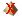
\includegraphics[width=0.7cm]{no_pyramid} This is a
%raster that has no pyramid layers (参见章 \ref{raster_pyramids}).\\
%
\includegraphics[width=0.7cm]{inoverview} This layer is
%shown in the overview map area as well as in the main map window.\\
%
\includegraphics[width=0.7cm]{editable} This is a vector
%layer that is currently enabled for editing.\\

\subsection{地图显示区}\label{label_mapview}
\index{map!view}

这是QGIS的“业务端点”——地图在这个区域显示!在这个窗口显示的地图将取决于所选择加载的图层(后续章节将会介绍如何加载图层)。地图视图可以平移和缩放(变换地图焦点到另一个地区)。其他各种操作可以如上述工具栏所描述的在地图上执行。地图视图和图例彼此紧密联系——图例区的改变会在视图中反映出来。

\begin{Tip}\caption{\textsc{使用鼠标滚轮缩放窗口}}\index{zoom!mouse wheel}
您可以使用鼠标滚轮缩放地图。将鼠标光标放到地图区域内向前滚动滚轮(远离您)放大地图,向后滚动(对着您)缩小地图。光标的位置就是缩放的中心。您可以通过 \mainmenuopt{设置} \arrow \dropmenuopt{选项} 下的菜单 \tab{地图工具} 来自定义鼠标滚轮缩放。
\end{Tip}

\begin{Tip}\caption{\textsc{使用方向键和空格键来进行地图平移}}\index{pan!arrow keys}
您可以使用方向键平移地图。把鼠标光标放在地图区域,敲击右方向键则地图向东平移,左方向键向西平移,上方向键向北平移,下方向键向南平移。您也可以用空格键平移地图:只需要按住空格键的同时移动鼠标即可。
\end{Tip}

\subsection{预览区地图}\label{label_mapoverview}
\index{map!overview}

地图全览面版提供了加载图层的完整范围的视图。可在 \mainmenuopt{设置} \arrow \dropmenuopt{面板} 菜单下选择地图概观。该视图是一个显示当前地图范围的矩形框。这使您可以快速确定当前正在查看的地图区。请注意即使在地图概观的图层已经设置标签,标签也不会在地图概观中显示出来。

您可以通过在图例窗口中右键点击图层,并选中 \checkbox{显示预览} 将一个单独的图层增加到地图概观中。您还可以通过工具栏中的概观工具来添加图层或移除概观中的所有图层。

如果在地图概观中单击并拖动显示当前范围的红色矩形框,地图的主要视图将会作出相应的更新。

\subsection{状态栏}\label{label_statusbar}

当鼠标指针在整个地图视图上移动时,状态栏显示出您在地图坐标系统中的当前位置(例如米或者十进制度数)。在状态栏显示坐标的左边是一个小按钮,用于显示坐标位置和显示平移与缩放地图范围之间的切换。

状态栏的进度条显示了每个图层添加到地图视图的渲染进度。在某些情况下,如在栅格图层统计数据收集,进度栏将被用于显示冗长的操作状态。

如果一个新的插件或者插件更新可用时,你会在状态栏看到消息。在状态栏右侧是一个小的复选框用于暂时阻止图层被渲染到地图视图(参见后面的章 \ref{subsec:redraw_events})。在状态栏的最右侧是一个投影图标。点击它打开当前项目的投影属性。

\begin{Tip}\caption{\textsc{计算您的地图区正确的缩放比例}}\index{scale!calculate}
当启动QGIS时,经纬度是默认的单位,它告诉QGIS图层的任何坐标都是用经纬度表示的。为了得到正确的缩放值,您可以在 \mainmenuopt{设置} \arrow \dropmenuopt{工程属性} 菜单下的 \tab{通用} 标签页中手动改成“米”,也可以在右下角状态栏处点击图标 \toolbtntwo{mIconProjectionDisabled}{projector} 。这样就可以根据工程投影的设定来确定地图单位,比如‘+units=m’
\end{Tip}

\subsection{键盘快捷键}\label{shortcuts}
\index{Keyboard shortcuts}

QGIS为许多功能提供了默认的快捷键,参见后面的 \ref{label_menubar} 。除此之外,菜单选项 \mainmenuopt{设置} \arrow
\dropmenuopt{自定义快捷键} 允许改变默认快捷键并为QGIS功能添加新的快捷键。

\begin{figure}[ht]
   \centering
   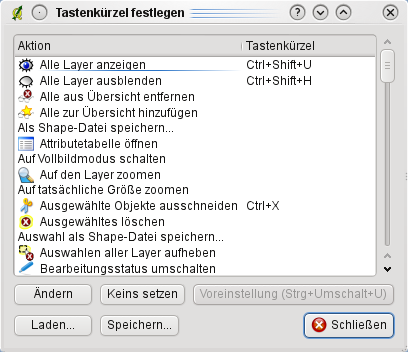
\includegraphics[clip=true, width=8cm]{shortcuts}
   \caption{自定义快捷键 \nixcaption (KDE)} \label{fig:shortcuts}
\end{figure}

自定义非常简单,只需从列表中选择一个功能并点击 \button{更改} , \button{取消快捷键} 或者 \button{设为默认} 。一旦用户建立了自己的配置,就可以将其存储为XML文件并加载到另一个QGIS装置。

\subsection{帮助上下文}\label{context_help}
\index{Context help}

当您需要特定主题的帮助时,可以通过在大部分对话框都可获得的Help按钮进入内容帮助——请注意第三方插件可以指向专门的网页。

\section{渲染}\label{subsec:redraw_events}\index{rendering}

默认情况下,每当地图画布必须被刷新的时候QGIS就会渲染所有可视图层。引发刷新地图画布的事件包括:

\begin{itemize}
\item 添加图层
\item 平移或缩放
\item QGIS窗口大小调整
\item 改变图层或图层集的可见度
\end{itemize}

QGIS允许用户用许多方式控制渲染过程。

\subsection{缩放相关的渲染}\index{rendering!scale dependent}
\label{label_scaledepend}

缩放相关的渲染可以指定每个图层可见的最小和最大比例。在图例显示区双击图层打开 \dialog{图层属性} 对话框可以设置缩放相关的渲染。在 \tab{通用} 标签页中,设置最小和最大比例值然后点击复选框 \checkbox{使用缩放相关的渲染} 即可。

用户可以通过缩放想要使用的水平并注意QGIS状态栏的缩放值来确定缩放数值。 \index{scale}

\subsection{地图渲染控制}\label{label_controlmap}

地图渲染可通过以下方式控制:

\minisec{a) 暂停渲染}\index{rendering!suspending}
\label{label_suspendrender}

在状态栏右下角点击 \checkbox{渲染} 复选框可暂停渲染。当 \checkbox{渲染} 复选框未选中时,QGIS都不会响应 \ref{subsec:redraw_events} 中所描述的任何事件来重绘画布。可能需要暂停渲染的例子有:

\begin{itemize}

\item 添加许多图层并更改其绘制的优先级
\item 绘图之前添加一个或者多个大图层并设置缩放比例
\item 绘图之前添加一个或者多个大图层并缩放至特定视图
\item 上述情形的任意组合
\end{itemize}

选中 \checkbox{渲染} 复选框可以渲染并且即使刷新地图画布。

\minisec{b) 设置图层添加的选项}\label{label_settinglayer}
\index{rendering!options}\index{layers!initial visibility}

用户可以设置一个选项,使之总是可以装载新的图层而不用绘图。这意味着该图层将被添加到地图中,但是其在图例窗口中的可见性复选框将默认为未选中。选择菜单选项 \mainmenuopt{设置}  \arrow \dropmenuopt{选项} 并点击 \tab{绘制 \& SVG} 标签页。取消选中 \checkbox{默认不显示新添加图层} 复选框之后,添加到地图的所有新图层都将默认关闭(不可见)。

%\minisec{Stopping Rendering}\index{rendering!halting}
%\label{label_stoprender}
%
%To stop the map drawing, press the ESC key. This will halt the refresh of
%the map canvas and leave the map partially drawn. It may take a bit of time
%between pressing ESC and the time the map drawing is halted.
%
%\textbf{NOTE}: It is currently not possible to stop rendering - this was disabled
%in qt4 port because of User Interface (UI) problems and crashes.

\minisec{c) 渲染时更新地图显示}
\label{label_updatemap}\index{rendering!update during drawing}

您可以在绘制图元时设置更新地图显示。默认情况下,QGIS不显示图层的任何要素直到全部图层被渲染。选择菜单 \mainmenuopt{设置} \arrow \dropmenuopt{选项} 项并点击 \tab{渲染 \& SVG} 标签,可对数据储存处读取的要素显示进行更新。将特征值设置为一个适当的值可在渲染过程中显示更新。将值设置为0将禁用绘图更新(这是默认值)。设置值过低会导致在读取要素过程中地图画布不断更新时较差性能。建议设置初始值为500。

\minisec{d) 影响渲染质量}
\label{label_renderquality}\index{rendering!quality}

有三个选项可影响地图的渲染质量。选择菜单选项 \mainmenuopt{设置} \arrow \dropmenuopt{选项},点击 \tab{渲染 \& SVG} 标签页,选中或取消选中以下复选框。

\begin{itemize}
\item \checkbox{牺牲部分绘制速度以提高线条抗锯齿}
\item \checkbox{修复多边形填充错误}
\end{itemize}

\section{量度}\label{sec:measure}\index{measure}

测量只能在投影坐标系中进行(例如 UTM)。如果加载的是一个地理坐标系(经/纬度)下的地图,那么线或区域的测量结果将是错误的。为了解决这个问题用户需要设置一个合适的地图坐标系统(参见节 \ref{label_projections} )。两种测量模块还使用了数字化模块捕捉设置。这对于在矢量图层沿着线或者区测量是有用的。

要选择测量工具,请单击 
\includegraphics[width=0.7cm]{mActionMeasure} ,然后选择需要的工具。

\subsection{长度、面积和角度量度}
\index{measure:line length}
\index{measure:areas}
\index{measure:angles}


\includegraphics[width=0.7cm]{mActionMeasure}
QGIS也可以依据定义的椭圆体测量给定点之间的实地距离。若要进行设置,选择菜单选项 \mainmenuopt{设置} \arrow \dropmenuopt{选项},然后点击 \tab{地图工具} 标签并选择适当的参考椭球体。也可在此处定义一个橡皮条颜色和首选测量单位(米或者英尺)。然后该工具就允许用户点击地图上的点。每段长度以及总长度都会显示在测量窗口。点击鼠标右键就可停止测量。 \\


\includegraphics[width=0.7cm]{mActionMeasureArea} 面积也可以量度。在测量窗口显示出累计的面积大小。此外,测量工具将捕捉到当前选中图层,该图层提供捕捉容限值设置(参见节 \ref{snapping_tolerance} )。所以,如果想测量精确的线要素或面要素首先设置其捕捉容限值,然后选中图层。那么当使用测量工具时,每个鼠标点击(在设置公差范围内)都将捕捉此图层。 \\


\includegraphics[width=0.7cm]{mActionMeasureAngle}
选中测量角度工具也可测量角度。光标变成十字形的。点击绘制您希望测量的的角度的第一段,然后移动光标绘制要求的角度。测量结果会显示在一个弹出的对话框。

\begin{figure}[ht]
\centering
   \subfloat[长度量度] {\label{subfig:measure_line}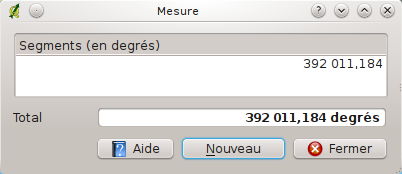
\includegraphics[clip=true, width=0.3\textwidth]{measure_line}}
     \hspace{0.33cm}
   \subfloat[面积量度]{\label{subfig:measure_area}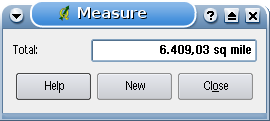
\includegraphics[clip=true, width=0.3\textwidth]{measure_area}}
     \hspace{0.33cm}
   \subfloat[角度量度]{\label{subfig:measure_angle}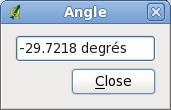
\includegraphics[clip=true, width=0.3\textwidth]{measure_angle}}
   \caption{实践中的量度工具 \nixcaption} \label{fig:measure}
\end{figure}

\subsection{选择和取消选择图元}\label{sec:selection}

QGIS 工具条上可以有好几种工具来选中地图显示区内的图元。要单选或多选图元,只需要单击 
\includegraphics[width=0.7cm]{mActionSelect} ,然后悬着工具:

\begin{description}
\item \radiobuttonon{选择图元}
\item \radiobuttonoff{矩形选择}
\item \radiobuttonoff{多边形选择}
\item \radiobuttonoff{自由形状选择}
\item \radiobuttonoff{半径选择}
\end{description} 

单击 
\includegraphics[width=0.7cm]{mActionDeselectAll} 可以取消所有图元的选择.

\section{工程}\label{sec:projects}\index{projects}

一个 QGIS 项目被组织成为一个工程。QGIS一次只能工作于某一个工程。工程属性或者是分工程设置,或者作为新工程的默认值进行设置(参见节 \ref{subsec:gui_options})。通过菜单 \mainmenuopt{文件} \arrow \dropmenuopt{mActionFileSave}{保存工程} 或者 \mainmenuopt{文件} \arrow \dropmenuopt{mActionFileSave}{工程另存为} 可以将您的工作空间保存为工程文件。

通过 \mainmenuopt{文件} \arrow \dropmenuopt{mActionFileSave}{打开工程} 或者  \mainmenuopt{文件} \arrow \dropmenuopt{mActionFileSave}{打开最近工程} 可以在 QGIS 会话中加载保存的工程文件。

如果您希望清空当前会话并重新开始,选择 \mainmenuopt{文件} \arrow \dropmenuopttwo{mActionFileNew}{新建工程} 。在打开或者最后一次保存一个工程后,如果工程文件已经被修改,那么以上各菜单选项都会提示您保存已有工程文件。

工程文件中保存的信息包括:

\begin{itemize}
\item 已添加的图层
\item 包括图例在内的图层属性
\item 地图的投影
\item 最后的视图范围
\end{itemize}

The project file is saved in XML format, so it is possible to edit
the file outside QGIS if you know what you are doing. The file format
was updated several times compared to earlier QGIS versions. Project files
from older QGIS versions may not work properly anymore. To be made aware of this,
in the \tab{General} tab under \mainmenuopt{Settings} \arrow \dropmenuopt{Options}
you can select: \\

\checkbox{Promt to save project changes when required} \\
\checkbox{Warn when opening a project file saved with an older version of QGIS}

\minisec{Project Properties}
In the properties window for the project under \nix{\mainmenuopt{File} \arrow
\dropmenuopt{Project Properties}} or \win{\mainmenuopt{Settings} \arrow
\dropmenuopt{Project Properties}} you set project specific options. These
include:

\begin{itemize}
\item In the \tab{General} tab the project title, selection and background
color, layer units, precision, and the option to save relative paths to
layers can be defined. In addition the topological editing, and layerwise
snapping options are set here.
\item The \tab{CRS} Coordinate Reference System tab enables you to choose the
CRS for this project, and to enable on-the-fly reprojection of vector layers
when displaying layers from a different CRS.
\item With the third \tab{Identifiable layers} tab you set (or disable) which
layers will respond to the identify tool. (See the Map tools paragraph from
the \ref{subsec:gui_options} section to enable identifying of multiple layers.)
\end{itemize}

\section{Output}\label{sec:output}
\index{output!save as image!print composer!quick print}

There are several ways to generate output from your QGIS session. We have
discussed one already in Section \ref{sec:projects}: saving as a project file.
Here is a sampling of other ways to produce output files:

\begin{itemize}
\item Menu option \dropmenuopttwo{mActionSaveMapAsImage}{Save as Image} opens
a file dialog where you select the name, path and type of image (PNG or JPG
format). A world file with extension PNGW or JPGW saved in the same folder
georeferences the image.
\item Menu option \dropmenuopttwo{mActionFilePrint}{Print Composer} opens a
dialog where you can layout and print the current map canvas (see
Section~\ref{label_printcomposer}).
\item The \toolbtntwo{quick_print}{Quick Print} plugin allows
to print a simple map with minimal effort (参见章 \ref{quickprint}).
\end{itemize}

\section{GUI Options}\label{subsec:gui_options}


\includegraphics[width=0.7cm,clip=true]{mActionOptions} Some basic options
for QGIS can be selected using the \dialog{Options} dialog. Select the
menu option \mainmenuopt{Settings} \arrow
\dropmenuopttwo{mActionOptions}{Options}. The tabs where you can
optmize your options are:

\minisec{General Tab}

\begin{itemize}
\item \checkbox{Promt to save project changes when required}
\item \checkbox{Warn when opening a project file saved with an older version of QGIS}
\item Change Selection and backgroud Color
\item Change the icon theme (choose between default, classic, gis and newgis)
\item \checkbox{Capitalise layer names in legend}
\item \checkbox{Display classification attribute names in legend}
\item \checkbox{Create raster icons in legend}
\item \checkbox{Hide splash screen at startup}
\item \checkbox{Open identify results in a dock window (QGIS restart
required)}
\item \checkbox{Open attribute table in a dock window}
\item \checkbox{Add PostGIS layers with double click and select in extended mode}
\item \checkbox{Add new layers to selected group}
\item Attribute table behavior (choose between Show all features (default), Show selected features,
show features in current canvas)
\end{itemize}

\minisec{Rendering \& SVG Tab}

\begin{itemize}
\item \checkbox{By default new layers added to the map should be displayed}
\item Define number of features to draw before updating the display.
\item \checkbox{Use render caching where possible to speed up redraws}
\item \checkbox{Make lines appear less jagged at the expense of some drawing
performance}
\item \checkbox{Fix problems with incorrectly filled polygons}
\item \checkbox{Use new generation symbology for rendering}
\item Add/remove path(s) to search for Scalable Vector Graphics (SVG) symbols
\end{itemize}

Additionally you can define wether to save the path for svg textures
absolute or relative in the \tab{General} tab of the
\mainmenuopt{Settings} \arrow \dropmenuopttwo{mActionOptions}{Project Properties}
menu.

\minisec{Map tools Tab}

\begin{itemize}
\item The Mode setting determines which layers will be shown by the Identify
tool. By switching to \usertext{Top down} or \usertext{Top down, stop at
first} instead of \usertext{Current layer} attributes for all identifiable
layers (see the Project properties section under: \ref{sec:projects} to set
which layers are identifiable) will be shown with the Identify tool.
\item \checkbox{Open feature form, if a single feature is identified}
\item Define search radius for identifying and displaying map tips as a
percentage of the map width
\item Define ellipsoid for distance calculations
\item Define rubberband color for measure tools
\item \radiobuttonon{Define preferred measurement units (meters or feet)}
\item \radiobuttonon{Define preferred angle units (Degrees, Radians or Gon)}
\item Define Mouse wheel action (Zoom, Zoom and recenter, Zoom to mouse
cursor, Nothing)
\item Define Zoom factor for wheel mouse
\end{itemize}

\minisec{Overlay}

\begin{itemize}
\item Define placement algorithm for labels (choose between central point
(standard), chain, popmusic tabu chain, popmusic tabu and popmusic chain)
\end{itemize}

\minisec{Digitizing Tab}

\begin{itemize}
\item Define Rubberband line color and line width
\item Define default snap mode (to vertex, to segment, to vertex and segment)
\item Define default snapping tolerance in map units or pixel
\item Define search radius for vertex edits in map units or pixel
\item \checkbox{Show markers only for selected features}
\item Define vertex marker style (cross (default), semi transparent circle or
none) and vertex marker size
\item \checkbox{Suppress attributes pop-up windows after each created feature}
\end{itemize}

\minisec{CRS Tab}

\begin{itemize}
\item \radiobuttonoff{Prompt for Coordinate Reference System (CRS)}
\item \radiobuttonoff{Project wide default Coordinate Reference System (CRS) will be used}
\item \radiobuttonon{Global default Coordinate Reference System (CRS) displayed below will be used}
\item Select global default Coordinate Reference System (CRS)
\end{itemize}

\minisec{Locale Tab}

\begin{itemize}
\item \checkbox{Overwrite system locale and use defined locale instead}
\item Information about active system locale
\end{itemize}

\minisec{Proxy Tab}

\begin{itemize}
\item \checkbox{Define timeout for network requests in ms}
\item \checkbox{Use proxy for web access} and define host, port, user, and password.
\item Set the \dropmenuopt{Proxy type} according to your needs
 \begin{itemize}
  \item \dropmenuopt{Default Proxy}: Proxy is determined based on the application proxy set using
  \item \dropmenuopt{Socks5Proxy}: Generic proxy for any kind of connection. Supports TCP, UDP, binding to a port (incoming connections) and authentication.
  \item \dropmenuopt{HttpProxy}: Implemented using the "CONNECT" command, supports only outgoing TCP connections; supports authentication.
  \item \dropmenuopt{HttpCachingProxy}: Implemented using normal HTTP commands, it is useful only in the context of HTTP requests
  \item \dropmenuopt{FtpCachingProxy}: Implemented using an FTP proxy, it is useful only in the context of FTP requests
 \end{itemize}
\end{itemize}

Excluding some URLs can be added to the textbox below the proxy-settings (see
fig. \ref{fig:proxy-settings}) by pressing the \button{Add}-button. After that
double-click into the just created URL-field and enter the URL you would like
to exclude from using the proxy. Obviously the button \button{Remove} removes the selected
entry.

If you need more detailed information about the different proxy-settings,
please refer to the manual of the unterlaying QT-library-documentation at
\url{http://doc.trolltech.com/4.5/qnetworkproxy.html#ProxyType-enum}.

\begin{figure}[ht]
   \centering
   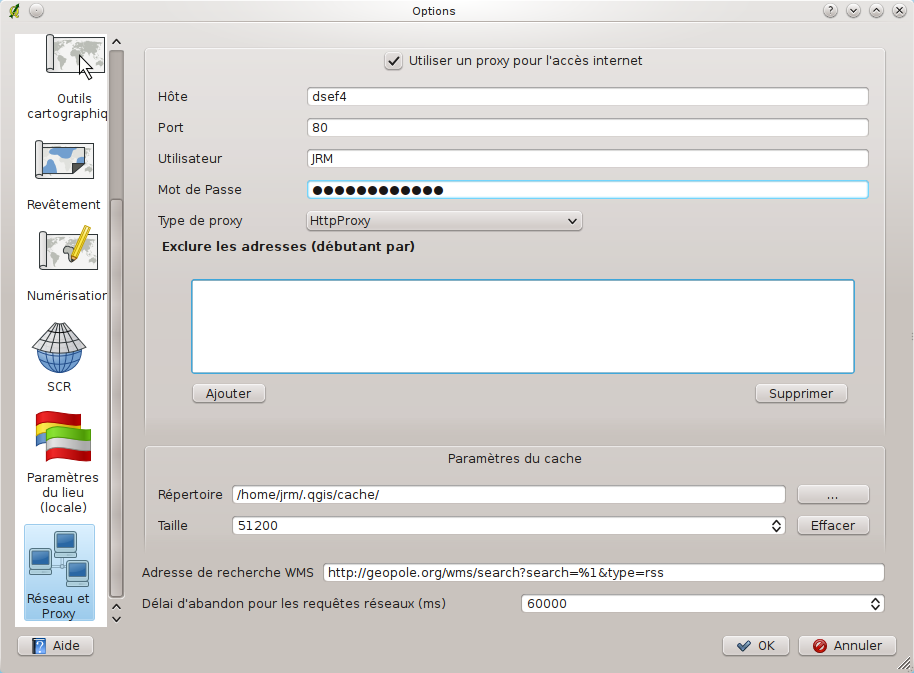
\includegraphics[clip=true, width=14cm]{proxy-settings}
   \caption{Proxy-settings in \qg \nixcaption}
   \label{fig:proxy-settings}
\end{figure}

\begin{Tip} \caption{\textsc{Using Proxies}}
Using proxies can sometimes be tricky. It is useful to 'trial and
error' the above proxy types and check if they succeed in your case.
\end{Tip}

You can modify the options according to your needs. Some of the changes may
require a restart of QGIS before they will be effective.

\begin{itemize}
\item \nix{settings are saved in a texfile: \$HOME/.config/QuantumGIS/qgis.conf}
\item \osx{you can find your settings in: \$HOME/Library/Preferences/org.qgis.qgis.plist}
\item \win{settings are stored in the registry under:}
\begin{verbatim}
\\HKEY\CURRENT\USER\Software\QuantumGIS\qgis
\end{verbatim}
\end{itemize}

\section{Annotation Tools}\label{sec:annotations}
\index{annotations}
\index{text annotation|\see{annotations}}

The 
\includegraphics[width=0.7cm,clip=true]{mActionTextAnnotation} text
annotation tools in the attribute toolbar provides the possibility to
place formated text in a balloon on the QGIS map canvas. Use the text
annotation tool and click into the map canvas.

\begin{figure}[ht]
   \centering
   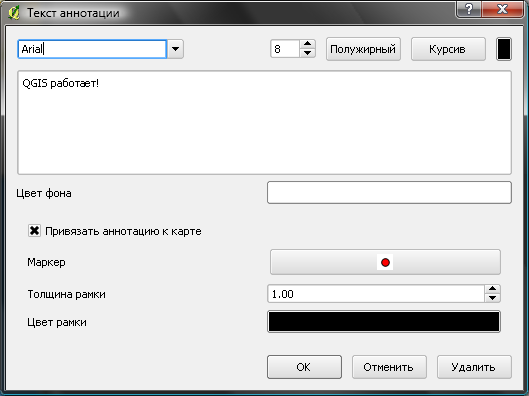
\includegraphics[clip=true, width=12cm]{annotation}
   \caption{Annotation text dialog \nixcaption}
   \label{fig:annotation}
\end{figure}

Double click on the item opens a dialog with various options. There is the
text editor to enter the formated text and other item settings. E.g. there
is the choice of having the item placed on a map position (displayed by
a marker symbol) or to have the item on a screen position (not related
to the map). The item can be moved by map position (drag the map marker)
or by moving only the balloon. The icons are part of gis theme, and are used
by default in the other themes too.

The 
\includegraphics[width=0.7cm,clip=true]{mActionAnnotation} move annotation
tool allows to move the annotation on the map canvas.

\subsection{Form annotations}\index{annotations}
\index{form annotation|\see{annotations}}

Additionally you can also create your own annotation forms. The

\includegraphics[width=0.7cm,clip=true]{mActionFormAnnotation} form annotation
tool is useful to display attributes of a vector layer in a customised qt
designer form (see Figure \ref{fig:custom-annotations}). It is similar to the
designer forms for the identify tool, but displayed in an annotation item.
Also see QGIS blog \url{http://blog.qgis.org/node/143} for more information.

\begin{figure}[ht]
   \centering
   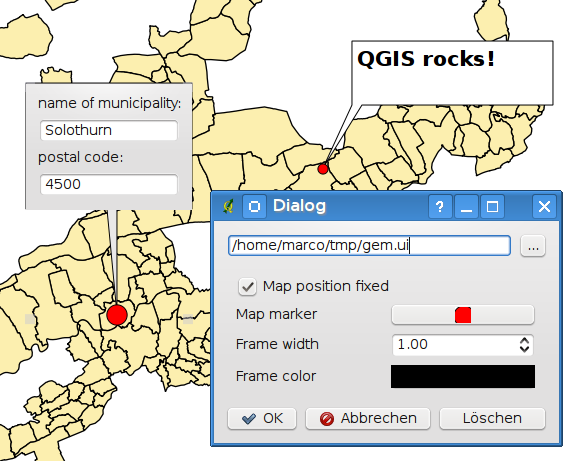
\includegraphics[clip=true, width=10cm]{custom_annotation}
   \caption{Customized qt designer annotation form \nixcaption}
   \label{fig:custom-annotations}
\end{figure}

\newpage

\section{Spatial Bookmarks}\label{sec:bookmarks}
\index{bookmarks}
\index{spatial bookmarks|\see{bookmarks}}

Spatial Bookmarks allow you to ``bookmark'' a geographic location and return to it later.

\subsection{Creating a Bookmark}
To create a bookmark:
\begin{enumerate}
\item Zoom or pan to the area of interest.
\item Select the menu option \mainmenuopt{视图} \arrow \dropmenuopt{New Bookmark} or press \keystroke{Ctrl-B}.
\item Enter a descriptive name for the bookmark (up to 255 characters).
\item Click \button{OK} to add the bookmark or \button{Cancel} to exit without adding the bookmark.
\end{enumerate}

Note that you can have multiple bookmarks with the same name.

\subsection{Working with Bookmarks}
To use or manage bookmarks, select the menu
option \mainmenuopt{视图} \arrow \dropmenuopt{Show Bookmarks}. The \\
\dialog{Geospatial Bookmarks} dialog allows you to zoom to or delete a bookmark.
You can not edit the bookmark name or coordinates.

\subsection{Zooming to a Bookmark}
From the \dialog{Geospatial Bookmarks} dialog, select the desired bookmark by clicking on it,
then click \button{Zoom To}.
You can also zoom to a bookmark by double-clicking on it.

\subsection{Deleting a Bookmark}
To delete a bookmark from the \dialog{Geospatial Bookmarks}
dialog, click on it then click \button{Delete}.
Confirm your choice by clicking \button{Yes} or cancel the
delete by clicking \button{No}.

\section{Live GPS tracking}\label{sec:gpstracking}

To activate Live GPS tracking in QGIS you need to select
\mainmenuopt{视图} \arrow \dropmenuopt{Live GPS tracking}. You will get a new
docked Window on the left side of the canvas.

There are 4 possible screens in this GPS tracking window
(see Figure \ref{fig:gpstrack_live} and Figure \ref{fig:gpstrack_options}).

\begin{description}
 \item[(a)] 
\includegraphics[width=0.5cm,clip=true]{mActionToggleEditing}
GPS position coordinates and for manually entering Vertices and Features
 \item[(b)] 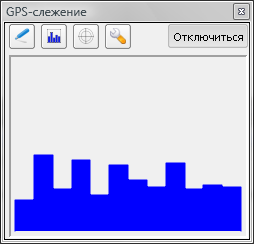
\includegraphics[width=0.5cm,clip=true]{gpstrack_barchart}
GPS signal strength of satellite connections
 \item[(c)] 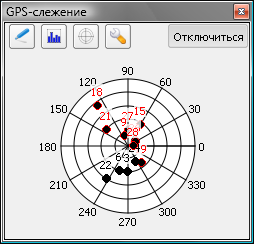
\includegraphics[width=0.5cm,clip=true]{gpstrack_polarchart}
GPS polar screen showing number and polar position of satellites
 \item[(d)] 
\includegraphics[width=0.5cm,clip=true]{mActionOptions}
GPS options screen (see Figure \ref{fig:gpstrack_options}).
\end{description}

With a plugged in GPS receiver (has to be supported by your operating system)
a simple click on \button{Connect} connects the GPS to QGIS. A second click
(now \button{Disconnect} disconnects the GPS-Reciever from you Computer. For 
GNU/Linux gpsd support is integrated to support connection to most GPS 
receivers. Therefore you first have to configure gpsd properly to connect QGIS to it.

[ IMPORTANT ]: If you want to record your position to the canvas you have to
create a new vector layer first and switch it to editable status to be able
to record your track.

\begin{figure}[ht]
\centering
   \subfloat[Position coordinates] {\label{subfig:gpstrack_main}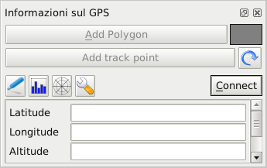
\includegraphics[clip=true, width=0.3\textwidth]{gpstrack_main}}
     \hspace{0.33cm}
   \subfloat[GPS signal strenght]{\label{subfig:gpstrack_stren}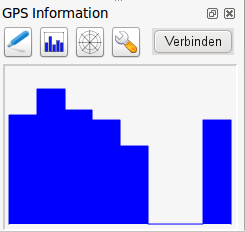
\includegraphics[clip=true, width=0.3\textwidth]{gpstrack_stren}}
     \hspace{0.33cm}
   \subfloat[GPS polar window]{\label{subfig:gpstrack_polar}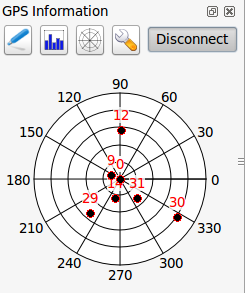
\includegraphics[clip=true, width=0.3\textwidth]{gpstrack_polar}}
\caption{Live GPS tracking \nixcaption} \label{fig:gpstrack_live}
\end{figure}

\begin{figure}[ht]
   \centering
   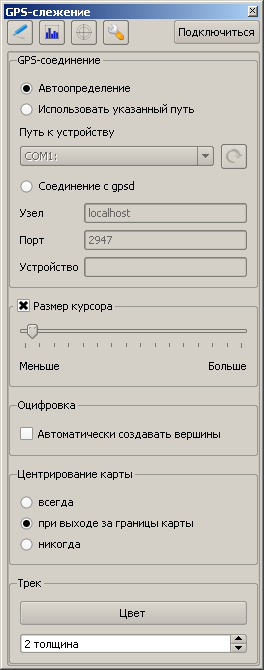
\includegraphics[clip=true, width=4cm]{gpstrack_options}
   \caption{GPS tracking options window \nixcaption}
   \label{fig:gpstrack_options}
\end{figure}

\subsection{Position coordinates}

\includegraphics[width=0.5cm,clip=true]{mActionToggleEditing} If the GPS is
recieving signals from satellites you will see your position in latitude,
longitude and elevation as you can see in Figure \ref{subfig:gpstrack_main}

\subsection{GPS signal strength}
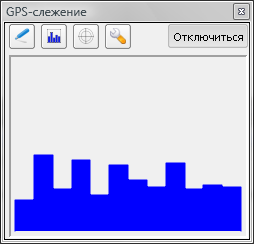
\includegraphics[width=0.5cm,clip=true]{gpstrack_barchart} Here you can see
the signal strenght of the satellites you are revieving signals from
(Figure \ref{subfig:gpstrack_stren}).

\subsection{GPS polar window}
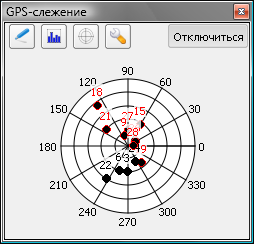
\includegraphics[width=0.5cm,clip=true]{gpstrack_polarchart} If you want
to know where in the sky all the connected satellites are, you have to
switch to the polar screen (Figure \ref{subfig:gpstrack_polar}).
You can also see the ID numbers of the satellites you are recieving signals from.

\subsection{GPS options}

\includegraphics[width=0.5cm,clip=true]{mActionOptions} In case of connection
problems you can switch from \radiobuttonon{Autodetect} to \radiobuttonon{Use
path/port below} and select the path/port your GPS receiver is connected to.
A click on \button{Connect} again initiates the connection to the GPS
receiver.

With the slider \slider{GPS Cursor Size} you can shrink and grow the position
cursor on the canvas. Activating \radiobuttonon{Auto-add vertices} within GPS
digitizing your track will automatically be recorded in the active vector layer
(of course the layer has to be in edit mode).

With GPS map recenter you can decide in which way the canvas will be
updated if your recorded coordinates start either to move out of canvas
or there is any change at all.

Track color and width sets the color of and the width of your drawn track.

If you want to set a feature manually you have to go back to

\includegraphics[width=0.5cm,clip=true]{mActionToggleEditing} ''Position Coordinates''
and click on \button{Add feature}. Also when you did not activate ''Auto-add vertices``
and want to record vertices manually you have to go back there and
click \button{Add vertex}

\FloatBarrier
